\documentclass[12pt]{article}

\usepackage{sbc-template}
\usepackage[utf8]{inputenc}
\usepackage{graphicx,url}
\usepackage[brazil]{babel}   
\usepackage[latin1]{inputenc}  
\sloppy

\title{Estrutura conceitual do Modelo para Agentes Normativos}

\begin{document} 

\section{Objetivo}

O modelo proposto tem como por finalidade representar atividades onde um grupo de pessoas  devem atuar de forma colaborativa com o propósito de resolver um problema. Esse problema pode ser dividido em etapas menores conhecidas como objetivos. Essas pessoas podem se relacionar entre sí, podem se relacionar com os artefatos presentes no meio 
onde elas atuam. Os artefatos também possuem a capacidade de se relacionar. Cada objetivo é concluído apenas se  um ou mais relacionamentos forem realizados. A conclusão do objetivo também é função de certos agentes e artefatos que devem ser presentes. 

Outra finalidade do modelo consiste em representar condições que devem ser mantidas ao longo da atividade, se essas condições forem desfeitas - a atividade deve ser encerrada de imediato, caso contrário as pessoas envolvidas nesta manutenção estarão submetidas a risco de morte. Dentro desta abordagem, alguém designado para cumprir com alguma atividade pode cometer erros. Esse modelo tem como por finalidade lidar com os seguintes tipos de erro: executar uma ação quando não há condições apropriadas para isso, manipular artefatos de maneira inapropriada ou inadvertida e escolher os artefatos inapropriados para cumprir com uma determinada atividade.

O modelo deve ser capaz de representar as consequências desses erros. Esse modelo está preocupado em representar dois tipos de consequências, essas são: 1 - imediatas que acontece sobre o indivíduo errante, 2 - a consequência manifesta em outro objetivo sobre o mesmo ou outro indivíduo pertencente ao grupo. Essas consequências são efeitos físicos negativos que alguém vêem a sofrer. A intensidade dessas consequências variam desde uma leve lesão a morte.

Outro aspecto deste modelo consiste representar objetivos cujo sucesso advem de certa característica aleatória presente na natureza da atividade. Essa característica aleatória consiste em um evento que possuem uma certa possibilidade de acontecer. Se esse evento acontecer, alguém sofre consequências ruins por conta disto. O modelo deve considerar relações entre erros onde as consequências se manifestam de forma indireta com eventos aleatórios.         

\section{Exemplo - Estudo de Caso}

Sete profissionais de linha viva (profissionais que realizam manutenção em equipamentos elétricos energizados) são designados com o propósito de realizar a substituição de um isolador de pedestal. Os papéis desses desses profissionais são; 1 supervisor, 1 observador e 5 executores. A manutenção de ve ser executada apenas sobre as seguintes condições: céu ensolarado e umidade relativa do ar menor que 70 porcento. Todos os profissionais devem possuir os EPIS necessários: capacete, óculos de sol, roupa isolante e anti-chamas, luvas isolantes e botas isolantes. Os profissionais que entrarão no potencial deverão estar vestidos de roupa condutiva e cabo guarda. As ferramentas necessárias para resolver esse problema são: bastão garra de diametro 64 x 3600 mm, sela de diametro 65 , colar, corda de fibra sintética, carretilha, chave com catraca, bastão universal, soquete adequado, locador de pino, bastão com soquete multiangular. A substitução do isolador de pedestal pode ser escrita nos seguintes subobjetivos: 


\begin{enumerate}
	\item Limpar, secar e testar corda.
	\item Instalar Bastão Garra na estrutura com o pedestal a ser substituído.
	\item Instalar sela com colar na estrutura
	\item Amarrar o bastão na parte superior da estrutura com a corda.
	\item Amarrar o olhal do bastão ao cavalo da sela atras de uma corda.
	\item Instalar um segundo conjunto bastão e sela no lado oposto da estrutura.
	\item Enforcar um estropo de Náilon no corpo do isolador.
	\item Colocar a extremidade do estropo no gancho da corda de serviço.
	\item Afrouxar os parafusos do conector que prendem a barra ao isolador.
	\item Terminar de retirar os parafusos com o bastão com o soquete multiangular.
	\item Elevar a barra através da corda que une a sela ao bastão.
	\item Apertar o colar através da porca borboleta.
	\item Segurar firmemente a corda de serviço.
	\item Sacar parafusos da base da coluna.
	\item Baixar o isolador ao solo
	\item Içar o Isolador
	\item Colocar Parafusos na base da coluna.
	\item Baixaer a barra para que a mesma apóie no novo isolador.
	\item Colocar os parafusos do conector que prende a barra ao novo isolador. 
	\item Retirar Equipamentos
\end{enumerate}

\section{Modelo}

\subsection{Definição dos Conjuntos}

\begin{enumerate}
	\item $Entity = \{e_1, ..., e_n\}$ - conjunto de todas as Entidades.  
	\item $Agent = \{ag_1, ..., ag_n\}$ - conjunto dos Agentes.
	\item $AgentGoal = agg = \{ag_1, ..., ag_n\}$ - conjunto dos Agentes que devem executar um determinado objetivo. 
	\item $Artefact = \{at_1, ..., at_n\}$ - conjunto dos Artefatos.
	\item $EntityGoal = eg = \{e_n,...,e_m\}$ - conjunto das Entidades que devem estar presentes para concluir um determinado objetivo $g_i$.
	\item $Relation = \{r_1, ..., r_n\}$ - conjunto dos Relacionamentos.	
	\item $RelationGoal = rg =\{r_n, ..., r_m\}$ - conjunto dos Relacionamentos que devem estar presentes para concluir um único objetivo $g_i$.		
	\item $Role = \{\rho_1, ..., \rho_n\}$ - conjunto dos Papéis.	
	\item $Goal = \{g_1, ..., g_n\}$ - conjunto dos Objetivos.
	\item $GoalRandomic = \{gr_1,..., gr_n\}$ - conjunto dos Objetivos	Randomicos.
	\item $GoalPrerequisit = gp = \{g_n,...,g_m\}$ - conjunto de Objetivos que são pré-requisitos para alcançar um outro objetivo.
	\item $Condition = \{c_1, ..., c_n\}$ - conjunto das Condições que devem ser mantidas ao longo da execução de todos os objetivos.
	\item $ConditionToGoal = cg = \{c_n, ..., c_m\}$ - conjunto de condições que devem ser mantidas para concluir um único objetivo $g_i$.
	\item $Risk = \{risk_1, ..., risk_n\}$ - conjunto dos Riscos na ocorrência de Eventos Ruins.
	\item $Possibility = \{p_1, ..., p_n\}$ - conjunto das possibilidades de Eventos Ruins. 
	\item $Fatality = \{f_1, ..., f_n\}$ - conjunto das fatalidades que acontecem na existência de um evento ruim. 	
\end{enumerate}


\subsection{Definição das Relações Entre os Conjuntos}

\begin{enumerate}
	\item $Entity \equiv Agent \cup Artefact$
	\item $Agent$ e $Artefact$ são disjuntos.
	\item $GoalRadomic \subset Goal$
	\item $\{agg_1,...,agg_n\} \subset Agent$	
	\item $\{gp_1,...,gp_n\} \subset Goal$
	\item $\{cg_1,...,cg_n\} \subset Condition$
	\item $\{eg_1,...,eg_n\} \subset Entity$		
	\item $\{rg_1,...,rg_n\} \subset Relation$	
\end{enumerate}

\subsection{Definição dos Predicados}

\begin{enumerate}
	\item $relationHas(r_l,e_i,e_k)$ onde $i \neq j$ - Um determinado relacionamento $r_l$ é composto por uma entidade $e_i$ e $e_k$ onde $e_i$ não pode ser igual a $e_j$.	
	\item $hasRole(ag_n,\rho_m)$ - Um determinado agente $ag_n$ tem um determinado papel $\rho_m$.
	\item $hasObligation(\rho_m,g_j)$ - Quem assume o papel $\rho_m$ é obrigado a concluir o objetivo $g_j$.
	\item $hasPermission(\rho_m,g_j)$ - Quem assume o papel $\rho_m$ tem a permissão de concluir o objetivo $g_j$.
	\item $isReached(g_k)$ - O objetivo $g_k$ foi alcançado.
	\item $stopIn(g_n,agg_m)$ - O objetivo não foi encerrado para todos os agentes que tiveram de executar. 	 				
	\item $stopIn(g_n)$ - A atividade como um todo teve de ser finalizada em $g_n$.	 			
	\item $isPreRequisite(gp_i,g_j)$ - Os objetivos $g$ pertencentes ao grupo $gp_i$ devem ser concluidos para que haja condição de executar g.
	\item $hasCondition(g_i,cg_n)$ - Um objetivo do tipo $g_i$ possui certas condições $c$ que deve estar presentes e devem se manter durante toda execução deste objetivo. Essas condições $c$ devem estar conditdas em $cg_n$. 
	\item $hasEntity(g_i,eg_i)$ - Um objetivo $g_i$ tem um conjunto de entidades $eg_i$ onde todas as entidades presentes neste conjunto devem estar presentes no momento da execução desse objetivo.
	\item $hasRelation(g_i,rg_i)$ - Um objetivo $g_i$ tem um conjunto de relacionamentos $rg_i$ onde todos esses relacionamentos devem ser feito para que este objetivo seja concluído.
	\item $isPresent(cg_n)$ - Todas as condições conditas em $cg_n$ estão presentes durante a tentativa de alcançar o objetivo.
	\item $isPresent(c_k)$ - Uma determinada condição $c_k$ está presente durante a tentativa de alcançar o objetivo.
	\item $isPresent(r_k)$ - Um determinado relacionamento $r_k$ está presente durante a tentativa de alcançar o objetivo.	
	\item $isPresent(e_k)$ - Uma determinada entidade $c_k$ está presente durante a tentativa de alcançar o objetivo.		
	\item $tryReach(ag_i,g_j)$ - Um determinado agente $ag_i$ tenta alcançar o objetivo $g_j$.
	\item $violationCondition(ag_i,g_j,c_k)$ - Um determinado agente $ag_i$ comete uma violação de condição no objetivo $g_j$ sobre a condição $c_k$. 
	\item $violationRelation(ag_i,g_j,r_k)$ - O agente $ag_i$ comete uma violação de Relacionamento no objetivo $g_j$ por não realizar o relacionamento $r_k$. 
	\item $violationEntity(ag_i,g_j,e_k)$ - O agente $ag_i$ comete uma violação de Entidade no objetivo $g_j$ por tentar alcançar esse objetivo sem ter a entidade $e_k$ presente.  	
	\item $hasRisk(c_k,risk_j,f_m)$ - A condição $c_k$ está associada a um risco $risk_k$ com uma certa fatalidade $f_m$. 
	\item $hasRisk(r_k,risk_j,f_m)$ - O relacionamento $r_k$ está associado a um risco $risk_k$ com uma certa fatalidade $f_m$.
	\item $hasRisk(e_k,risk_j,f_m)$ - A entidade $e_k$ está associada a um risco $risk_k$ com uma certa fatalidade $f_m$.
	\item $consequenceOfBadEvent(g_k,ag_i,risk_j,f_m)$ - Agente $ag$ sofre as consequências do risco $risk_j$ com a fatalidade $f_m$
	\item $hasPossibility(gr_n,p_m)$ - Possibilidade $p_m$ do evento $gr_n$ gerar alguma consequência ruim. 	
	\item $affects(r_k,gr_n,p_n)$ - Se uma relação $r_k$ não for feito, ou se essa relação for mal feita, então ela afeta negativamente algum objetivo com carater aleatório mudando a possibilidade para $p_n$ de um evento ruim acontecer. 	
	\item $happensBadEvent(gr_n,r_m,ag_k)$ - O evento ruim de $g_r$ acontece em relação a um relacionamento necessário sobre um agente $ag_k$. 		
\end{enumerate}

\subsection{Definição das Relações de Implicabilidade}

Todo agente que é obrigado a alcançar um determinado objetivo deve ter a permissão para realizar essa ação.
\begin{equation}\label{rel1}
	hasObligation(\rho_m,g_j) \to hasPermission(\rho_m,g_j)  
\end{equation}

Um agente que tenta alcançar um objetivo sem que pelo menos uma das condições necessárias para isso esteja presente, comete uma violação conhecida como violação de condição.
\begin{eqnarray}\label{rel3}\nonumber
	hasCondition(g_i,cg_n) \wedge \neg isPresent(c_k) \wedge (c_k \in cg_n) \wedge tryReach(ag_m,g_i) \to \nonumber \\  
	violationCondition(ag_m,g_j,c_k) \wedge \nonumber \\
	hasCondition(g_i,cg_n) \wedge isPresent(cg_n) \wedge tryReach(ag_m,g_i) \to \nonumber \\  
	\neg violationCondition(ag_m,g_j,c_k)  	
\end{eqnarray}

Se um agente não executa, ou não tem condições de executar, um dado relacionamento $r_k$ necessário para concluir o objetivo, então o agente cometeu uma violação de relacionamento. Contudo, se o agente alcançar o objetivo, então a não violação acontece. 
\begin{eqnarray}\label{rel4}\nonumber
	hasRelation(g_i,rg_n)\wedge \neg isPresent(r_k)  \nonumber \\ 
	\wedge (r_k \in rg_n) \wedge tryReach(ag_m,g_i) \to violationRelation(ag_m,g_i,r_k) \nonumber \\
	\wedge \nonumber
	\\
	hasRelation(g_i,rg_n)\wedge isPresent(rg_n)  \nonumber \\ 
	 \wedge tryReach(ag_m,g_i) \to  \neg violationRelation(ag_m,g_i,r_k) 
\end{eqnarray}

Se ao tentar alcançar um determinado objetivo pelo menos uma das entidades necessárias para isso está ausente, então acontece um uma violação de entidade. Contudo, se todas as entidades estiverem presente, então a vioalação não acontence. 
\begin{eqnarray}\label{rel5}\nonumber
	hasEntity(g_i,eg_n) \wedge \neg isPresent(e_k) 	\wedge (e_k \in eg_n) \wedge tryReach(ag_m,g_i) \to \nonumber \\ violationEntity(ag_m,g_i,e_k) \nonumber \\
	hasEntity(g_i,eg_n) \wedge  isPresent(eg_n) \wedge tryReach(ag_m,g_i) \to \nonumber \\ \neg violationEntity(ag_m,g_i,e_k)  
\end{eqnarray}


Uma violação de condição tem como consequêcias a ocorrência do risco (sobre o agente que cometeu a violação) relacionado a condição que não estava presente. Esse risco pode apresentar diferentes graus de fatalidade.
\begin{eqnarray}\label{rel9}\nonumber
	violationCondition(ag_m,g_i,c_k)  \wedge hasRisk(c_k,risk_j,f_m) \to \\ 
	consequenceOfBadEvent(g_i,ag_m,risk_j,f_m)
\end{eqnarray}

Uma violação de relacionamento tem como consequência a ocorrência do risco (sobre o agente que cometeu a violação) relacionado ao relacionamento que não foi feito. Esse risco pode apresentar diferentes graus de fatalidade.
\begin{eqnarray}\label{rel10}\nonumber
	violationRelation(ag_m,g_i,r_k) \wedge hasRisk(r_k,risk_j,f_m) \to \\ 
	consequenceOfBadEvent(g_i,ag_m,risk_j,f_m)
\end{eqnarray}

Uma violação de relacionamento tem como consequência o aumento da possibilidade de acontecer algo de errado em objetivos que podem ser afetados por características aleatórias. Assim sendo, esse outro objetivo tem uma nova possibilidade de dar errado que é necessariamente maior a possibilidade antiga.
\begin{eqnarray}\label{rel11}\nonumber
	violationRelation(ag_m,g_i,r_k) \wedge affects(r_k,gr_n,p_n) \wedge hasPossibility(gr_n,p_m) \to \\  
	hasPossibility(gr_n,p_n) \wedge (p_n > p_m)
\end{eqnarray}

Uma violação de entidade gera a interrupção imediata da atividade no objetivo de ocorrência.
\begin{eqnarray}\label{re12}
	violationEntity(ag_m,g_i,e_k) \to stopIn(g_i)
\end{eqnarray}

Em um objetivo onde existe uma certa possibilidade de dar errado, essa possibilidade é vinculada aos relacionamentes que devem ser feitos para concluir este objetivo. Assim sendo, um determinado agente sofrerá as consequêcias ruins pela ocorrência do evento.
\begin{eqnarray}\label{rel13}\nonumber
	happensBadEvent(gr_n,r_m) \wedge hasRisk(r_k,risk_j,f_m) \nonumber \\ 
	\to consequenceOfBadEvent(gr_n,ag_m,risk_j,f_m)
\end{eqnarray}

A ocorrência de um evento ruim gera imediata interrupção das atividades.
\begin{eqnarray}\label{rel14}
	consequenceOfBadEvent(g_k,ag_m,risk_j,f_m) \to stopIn(g_k)
\end{eqnarray}

Se o objetivo não é encerrado para todos os agentes que tinha como por permissão executa-lo, então o objetivo é alcançado. 
\begin{eqnarray}\label{rel15}
	\neg stopIn(g_k,agg_n) \to isReached(g_k)
\end{eqnarray}


\subsection{Justificando a Existência das Relações de Implicabilidade}

\subsubsection{Relação \ref{rel1}}
A relação \ref{rel1} existe com base em estudos sobre lógica deontica (definir o estudo) onde um indivídulo só pode ser obrigado a fazer algo se esse indivídulo tiver permissão para isso. Caso contrário, há uma contradição em relação a semântica dos predicados, pois é dado como absurdo alguém ser obrigado a fazer algo sem ter permissão para isso. 


\subsubsection{Relação \ref{rel3}}

Representar condições que devem ser mantidas ao longo de toda a execução da atividade bem como as consequências de praticar uma determinada atividade dado a ausência de pelo menos uma das condições é um aspecto sobre o qual este modelo se propõem a representar. Para definir a ocorrência da vioação se faz necessário saber quais são as condições vinculadas ao objetivo, pois caso contrário não é possível identificar quais condições devem ser mantidas ao longo da tentativa de se alcançar um objetivo e, por consequência, qualquer afirmação feita sobre essas condições não possui uma sustentação lógica rigorosa. A consideração dessas relações acontece por meio predicado $hasCondition(g_i,cg_n)$. 

Outro aspecto relevante consiste saber se a condição necessária para tentar alcançar o objetivo não está presente durante a tentativa. Se isso não for feito, não é possível saber se a condiçõe está presente durante a tentativa de alcançar o objetivo e qualquer afirmação derivada das condições não apresenta sustentação lófica. Isso é feito por intermédioo do predicado $isPresent(c_k)$. Ao saber que é verdade o negado de $isPresent(c_k)$, é possível saber que a condição $c_k$ não está presente. Ainda sim, definir em uma única expressão o predicado $hasCondition(g_i,cg_n)$ e o predicado $isPresent(c_k)$ não é o suficiente, pois $cg_n$ é um conjunto e $c_k$ é um elemento que pode ou não pertencer ao conjunto $cg_n$. Assim sendo, isso deve ser levado em consideração por agregar a seguinte relação a expressão: $c_k \in cg_n$. 

Os predicados considerados até o momento são necessários, porém não são suficientes. Isso, pois apenas com eles não é possível definri qual é a situação do agente em relação ao objetivo. Por exemplo, é possível considerar um cenário onde pelo menos uma das condições necessárias para atingir o objetivo não está presente. Contudo, não é razoável, considerando o conceito de violação de condição empregado neste estudo, afirmar que o agente cometeu uma violação de condição sobre esse cenário sendo que não há informaçãoa sobre a situação da tentativa do agente alcançar o objetivo. Assim sendo, se o agente tentar alcançar o objetivo mesmo com pelo menos uma condição inexistente, então esse agente cometeu uma violação de condição, contudo se o agente não tento alcançar o objetivo em análise então ele não cometeu violação alguma. Então, a informação no que diz respeito ao gente é deve ser considerada nessa relação de implicabilidade e isso acontece por meio do predicado $tryReach(ag_m,g_i)$.

Para definir a ausência de violação, todas das condições devem estar presentes. Para representar isso, a relação \ref{rel3} exibe uma segunda relação de implicabilidade que consdera o negado de uma violação de condição dada a presenção de todas as condições necessárias para o objetivo. 

 
\subsubsection{Relação \ref{rel4}}
Para levar em consideração violações sobre se o agente sabe ou não manipular algum tipo de relação, se faz necessário buscar por relações de implicabilidade que verificam as seguintes circunstâncias: relações que devem ser feitas para que um determinado objetivo possa ser atingido $hasRelagion(g_i,rg)$, se a relação em análise é uma relação que pertence a todas as relações necessárias para findar esse objetivo $r_k \in rg_g$, vericar se a relação em análise está presente quando o agente realiza a atividade $isPresent(r_k)$ e levar em consideração o ato do agente tentar executar a atividade $tryReach(ag_m,g_i)$.  A violação acontece quando, na reunião de todas essas circunstâncias, uma das relações não se faz presente $\neg isPresent(r_k)$. Para essa situação, $violagionRelation(ag_m,g_i,r_k)$ tem que ser verdadeiro. Se todas as relações $rg_n$ estão presentes, então a violação de relação não acontece e isso é formalizado por meio da segunda relação de implicabilidade presente na \rel{rel4}. 

Considerando que uma violação de relacionamento acontece quando um agente tenta alcançar um objetivo sem realizar um ou mais dos relacionamentos necessários para que esse objetivo seja satisfeito com sucesso, é possível demonstrar a necessidade das circunstâncias presentes na relação de implicabilidade deste modelo por analisar o que acontece na ausência de cada uma delas. Seguindo por essa linha, supondo uma situação onde não se verifica as relações relevantes para um objetivo, logo não é possível dizer se a ausência de uma violação em específico é relevante para o objetivo em análise. Assim sendo, não é possível afirmar quando acontece uma determinada vioalação. 

Supondo uma situação onde não se verifica as relaçõeas que foram concluidas durante o ato da manutenção. Neste cenário é possível saber quais relações são necessárias para alcançar um determinado objetivo, mas deste conjunto não é possível definir qual dessas relações foram alcançadas. Se não se sabe afirmar qual das relações um agente conseguiu realizar, não se sabe qual dessas relações um agente deixou de fazer. Não sabendo esta ultima, não se sabe se ocorreu uma violação dessa relação. Assim sendo, só é possível afirmar algo sobre a ocorrência de uma vioalação de relação se for possível analisar se as relações necessárias para um dado objetivo foram ou não cumpridas. 

Supondo uma situação onde não se verificar se um agente tentou realizar o objetivo. Nesta situação não é possível analizar quem cometeu a violação. Além disso não é possível considerar se a presença ou a ausência das relações são relevantes ou não para alcançar o objetivo, pois não se pode localizar a ocorrência dessas relações nos momentos onde elas devem acontecer (que é quando o agente tenta alcançar o objetivo dessas relações). Além disso, desconsiderar a tentativa do agente envolve descaracterizar a ocorrência da violação uma vez que esta, por conseguinte, considera a existência de um agente durante a ocorrência de uma violação. 

\subsubsection{Relação \ref{rel5}}

Para verificar violações onde um agente tenta executar um determinado procedimento sem ter todas entidades (ex. ferramentas, colegas) para isso, é necessário construir uma expressão de implicabilidade que consider quais são as entidades importantes para a execução do objetivo $hasEntity(g_i,eg_n)$, considere quais as entidades que estão presentes no ambiente durante o ato da execução $isPresent(eg_n)$,$isPresent(e_k)$,$e \in eg_n$ e que considere se um agente tentou alcançar o objetivo $tryReach(ag_m,g_i,e_k)$. Para situação onde está ausente uma das entidades necessárias para concluir um dado objetivo, então acontece uma vioação de entidade. Contudo, para situação onde todas as entidades necessárias para alcançar um objetivo estão presentes durante a tentativa que o agente tem para isso, então a violação não acontence. 

Se uma vioalação de entidade é definida como sendo a tentativa de um agente alcançar um determinado objetivo sem ter todas as entidades para isso, então é possível verificar e necessidade de todas as circunstâncias por analisar o que acontece na ausência delas. Supondo não ser possível verificar quais entidades são necessárias para alcançar um determinado objetivo, então não é possível afirmar quais entidades devem ser presentes durante a tentativa do agente em alcançar um determinado objetivo. Por consequência, também não é possível identificar quais entidades estão ausentes logo, neste caso é um absurdo fazer qualquer afirmação sobre presença ou ausência sobre violação por ausência de uma entidade. Supondo não ser possível afirmar se uma entidade necessária para conclusão de um determinado objetivo não está presente durante a tentativa de alcançar esse objetivo. Então, é um absurdo afirmar que aconteceu ou não aconteceu um evento no que diz respeito a ausência de uma entidade sem mesmo saber se essa entidade estava presente. Suponto não ser possível definir se um agente tentou ou não executar o objetivo. Então também não é possível saber se a entidade estava presente no momento em que deve estar presente para definir a ocorrência de uma violação, além de descaracterizar a semântica da violação de uma entidade usada por este modelo uma vez que está considerar necessariamente a existência de um agente pela ocorrência da violação. 


\begin{figure}
  \centering
  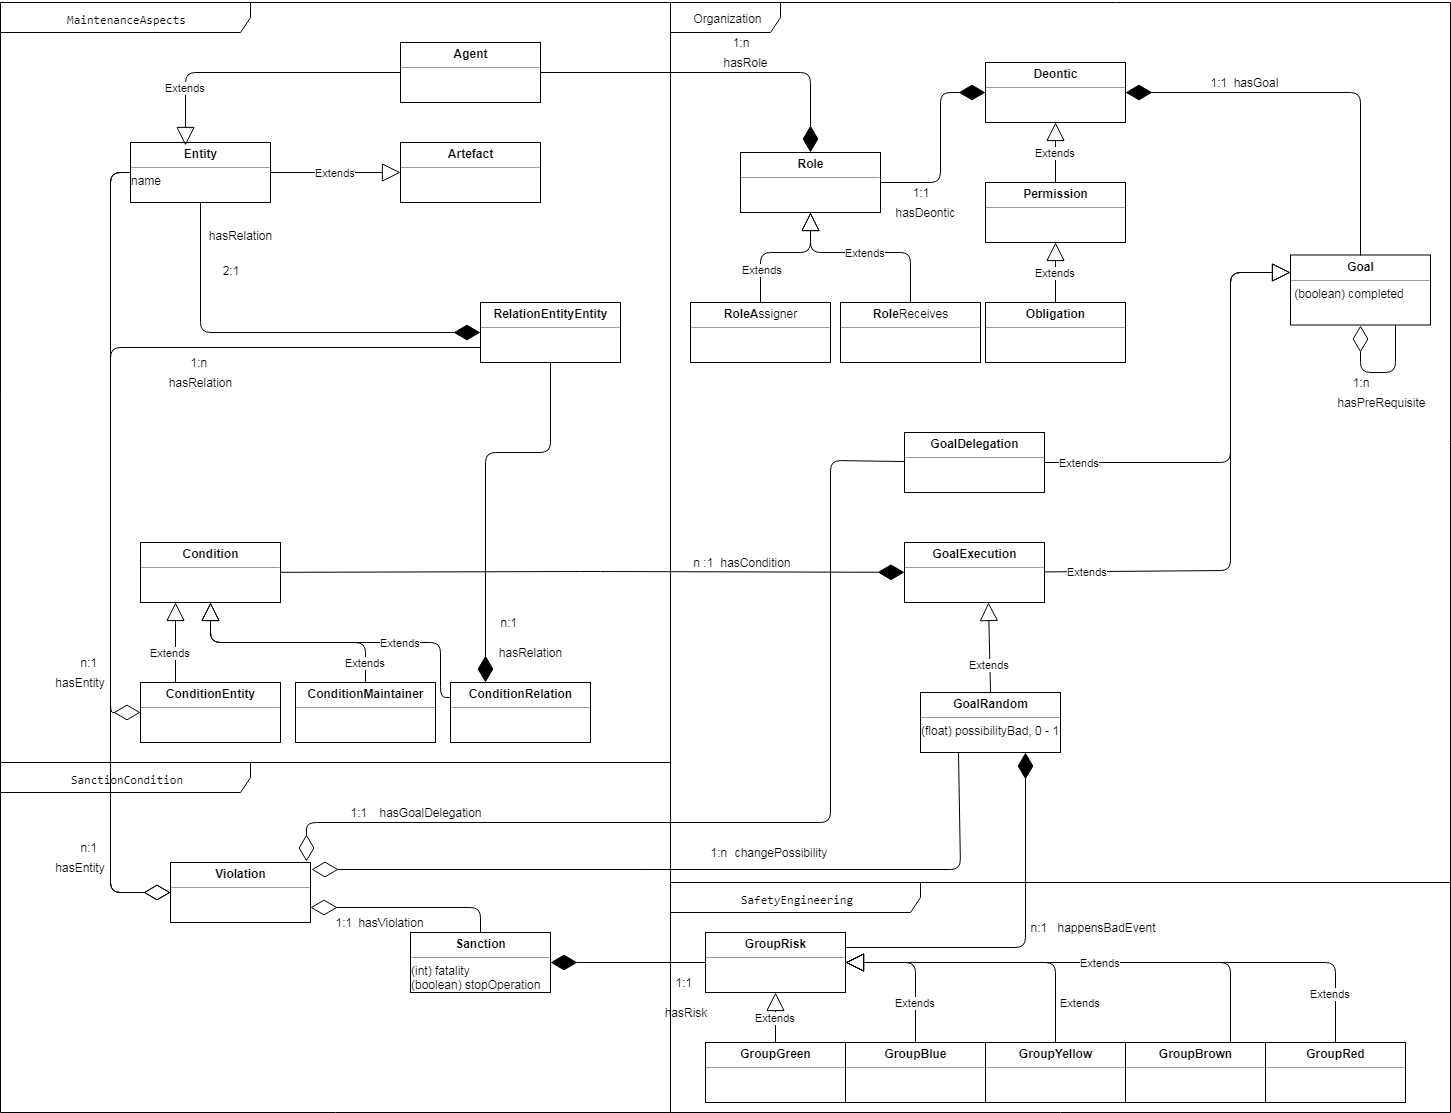
\includegraphics[width=0.8\linewidth]{umlmodel} 
\end{figure}

\end{document} 
